% Clase del documento
\documentclass[a5paper, 12pt]{article}

% Paquetes
\usepackage[utf8]{inputenc}
\usepackage[spanish, es-nolayout, es-nodecimaldot, es-tabla]{babel}
\usepackage[top=2cm, left=2cm]{geometry}
\usepackage{amsmath, amssymb, amsfonts, latexsym}
\usepackage{graphicx}
\usepackage[x11names,table]{xcolor}
\usepackage{multicol}
\usepackage{multirow}
\usepackage{caption}
\usepackage{url}
\usepackage[colorlinks = true, filecolor=magenta, urlcolor=magenta,]{hyperref} 

% Comandos
\parindent = 0mm

\author{Milton Torres \and Andrés Mt}

\title{Holi}

\date{\today}


\definecolor{db}{RGB}{0,128,128}
\definecolor{dh}{RGB}{128,128,0}

% Contenido
\begin{document}
	\maketitle

	Cualquier cosa dijo                                                                                                                                                                Milton y no sabía que yo iba a refutarle absolutamente todo, todo lo que iba a decir :D
	
{	\color{yellow}Cualquier cosa dijo Milton y no sabía que yo iba a refutarle absolutamente todo, todo lo que iba a decir :D}
Cualquier cosa dijo Milton y no sabía que yo iba a refutarle absolutamente todo, todo lo que iba a decir :D

Cualquier cosa dijo Milton y no sabía que yo iba a refutarle absolutamente todo, todo lo que iba a decir :D


%\vspace{-1\baselineskip}
\setlength{\columnsep}{30pt}
\begin{multicols}{2}
		Annie Hall is a 1977 American romantic comedy film directed by Woody Allen from a screenplay he co-wrote with Marshall Brickman.
		
		 Produced by Allen’s manager, Charles H. Joffe, the film stars the director as Alvy "Max" Singer, who tries to figure out the reasons for the failure of his relationship with the film’s eponymous female lead, played by Diane Keaton in a role written specifically for her.
\end{multicols}
	
	Salté la línea.
	
	\section[EPN]{Escuéla Politécnica Nacional}
	
	\subsection{La historia de la patata mística}
	\subsubsection{Y Milton}
	
	\textbackslash Po\hspace{2\baselineskip}rque m\qquad uchos back\quad slash son div\, ersión to\ tal. \^{}
	
	
	\textbf{\emph{hola}}	

	\begin{itemize}
		\item Mi texto 1
		\item Mi texto 2
	\end{itemize}        
ejemplo con espacio
	
	\begin{enumerate}
		\item Mi texto 1
		\item Mi texto 2
		
		\begin{enumerate}
			\item Hola 1
			\item Hola 2
			
			\begin{itemize}
				\item Oh no
				
				\begin{description}
					\item[Milton:] Aw
					\item[Andrés:] oh
				\end{description}								
				
			\end{itemize}
			
			\item Hola 3
		\end{enumerate}
		
		\item Mi texto 3
	\end{enumerate}

	
	
	\emph{Algo de texto negro, \color{red} seguido por un fragmento rojo}, {\color {blue} finalmente algo de texto azul.}
%
%
%
	
	\centerline{Lea esta frase, por favor.}


	
	\begin{center}
	
		Esto lo escribí yo.
		
	\end{center}	

\begin{flushright}
   There are two types of people in this world, good and bad. \\
   The good sleep better, but the bad seem to enjoy \\
   the waking hours much more. \\
   \textbf{Woody Allen (director neoyorquino)}
\end{flushright}

	
	
	\begin{center}
		<<There are two types of people in this world, good and bad. The good sleep better,
		
		but the bad
         seem to enjoy the waking hours much more.>>
		\emph{Woody Allen}
\end{center}	
	
	
	{\tiny
	Cualquier cosa dijo                                                                                                                                                                Milton y no sabía que yo iba a refutarle absolutamente todo, todo lo que iba a decir :D}
	
	cual cosa
	
	{\Huge GRANDE}
	
	

	\begin{center}
		\begin{tabular}{r @{Lipton} l} %Para alinear y poner lo que quiero eque este entre la mitad {.}
		\hline
		\(1\) & \(4\) \\ \hline \(2\) & \(54\) \\ \hline \(1\) & \(7890\) \\ \hline
	   \end{tabular}
	\end{center}
	
	
\begin{center}
   \begin{tabular}{ |l|l|l| }
		\hline
		\multicolumn{3}{ |c| }{Team sheet} \\
		\hline
		Goalkeeper &
		\multicolumn{2}{|c|}{Nom}
%		 GK & Paul Robinson 
		 \\ \hline
		\multirow{4}{*}{Defenders} & LB & Lucus Radebe \\ 	%\multirow: para combinar filas
	                                               & DC & Michael Duburry  \\
    	                                           & DC & Dominic Matteo  \\
	                                               & RB & Didier Domi  \\
    	  \hline
		\multirow{3}{*}{Midfielders} & \multirow{3}{*}{MC} & David Batty \\ 
		                                           &                                 & Eirik Bakke \\
	                                               &                                 & Jody Morris \\
		\hline
		Forward                              & FW                          & Jamie McMaster \\ \hline 
		
    \multirow{2}{*}{Strikers} & \multirow{2}{*}{ST} & Alan Smith \\ 
		                                  &                                & Mark Viduka 		\\
		\hline
   \end{tabular}
\end{center}	

\newpage

\begin{table}[h]
	\captionsetup{font=footnotesize}
	\centering
	\scalebox{0.75}
	%
	{
		\begin{tabular}{|c|c|c|} \hline
			\(p\) & \(q\) & \(p \to q\) \\
			\hline
			0&0&1 \\
			0&1&1 \\
			\cline{1-2}
			1&0&0 \\
			1&1&1 \\
			1&1&1 \\
			1&1&1 \\
			1&1&1 \\
			1&1&1 \\
			1&1&1 \\
			1&1&1 \\
			1&1&1 \\
			1&1&1 \\
			1&1&1 \\
			1&1&1 \\
			1&1&1 \\	
			1&1&1 \\
			\hline
		\end{tabular}
	%
	}
	\caption{Tabla de verdad para \(p \to q\).}
	\label{tabla:01}
\end{table}
Esta es la tabla \ref{tabla:01}


	
\begin{center}
	\begin{tabular}{| >{\columncolor{db!20}} c | c  | >{\color{magenta}} c |}
		\hline
		\rowcolor{red!75}
		\color{yellow!30!white} \textbf{Temperatura} &
		\color{yellow!30!white} \textbf{Tiempo} &
		\color{yellow!30!white} \textbf{Total} \\ \hline
		1 & \(245 \pm 5.5\) & 3 \\ \hline
		2 & \(260 \pm 5.5\) & \cellcolor{white!70!dh}\color{dh}{8} \\
		 \hline % para pintar una sola celda
		 3 & \(275 \pm 5.5\) & 8 \\ \hline
		 4 & \(287 \pm 5.5\) & 8 \\ \hline
	\end{tabular}
\end{center}
	
	\includegraphics[scale=0.45]{El_grafico}
	
	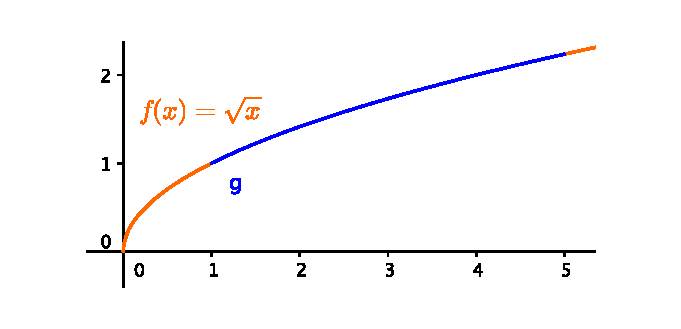
\includegraphics[scale=1]{El_grafico_2}
	
	
\end{document}

jhafodhfaqnlna aefhjalfjnali fah